\documentclass{article}
\usepackage[utf8]{inputenc}
\usepackage{amsmath}
\usepackage{amssymb}
\usepackage{enumitem}
\usepackage{bm}
\usepackage{graphicx}
\usepackage{float}
\usepackage{caption}
\usepackage{subfig}
\usepackage{array}
\usepackage{wrapfig}
\usepackage{multirow}
\usepackage{tabu}
\usepackage[framed,numbered,autolinebreaks,useliterate]{mcode}
\begin{document}

\title{Indepedent Study report}
\author{Xin Bai}
\date{}
\maketitle
\section{Introduction}

There are three sources that limit the resolution of CT image. They are the size the light source, the photon diffusion and the pixel size of the detector.  We focus on solving the image resolution problem caused by the pixel size of the detector in this report. 

According to Nyquist sampling theorem, a continuous signal can be fully reconstructed if it was sampled using the frequency that is twice the highest frequency that signal contains. However, due to the limited size of the pixel, the sampling rate is limited, thus it is unable to capture some high frequency information. And this will lead to the aliasing in the image. 

This report implements a dealiasing method which uses a sequence of low-resolution image with small movement to try to estimate a high-resolution image. The relative movement should be smaller than the size of the pixel. With the , we can build a linear relation between the high resolution image and low resolution image. So we can reconstruct the high-resolution image.

\section{Method}
The idea for reconstruction is that the low resolution image could be obtained by downsampling the high resolution image. To be more explicitly, each low resolution pixel could be viewed as the weighted-averaging result of the corresponding high resolution pixel. The relation could be described as:
	\begin{align}
		y = Az + n
	\end{align}
	\begin{align}
		y_{i}=\Sigma_{N}w(s)_{n}z_{n}
	\end{align}
, in which $z$ represents the high resolution image, $y$ is the low resolution image and $A$ is the coefficient matrix that specify the contribution pixel for each low-resolution pixel, $n$ is the nosie, $i$ is a pixel in low-resolution image, $N$ is the total number of pixels in $y$, and $w_n$ denotes the contribution of each high-resolution pixel to $y_i$ and . For $y$ that have relative movement to $z$, partial contribution should be considered, whose value depends on overlap between moving image and still image. The parameter $s$ in $w(s)$ reflect this situation. 

However, due to the errors in mechanics, the real movement does not equal the stage shift as we acquire the data image. We can use MAP method to estimate the best result of high resolution image $z$ and the movement parameters $s$. So our goal becomes find $\hat{z}$ and $\hat{s}$ that maximizes the $P(z,s|y)$. Next we assume $z$ has a Gaussian prior, the final cost function could be written as : 
	\begin{align}
		L(z,s) = \frac{1}{2\sigma_n^2}(y-W_sz)^T(y-W_sz)+\frac{1}{2}z^TC_z^{-1}z
	\end{align}
$\sigma$ is the variance of the Gaussian noise, $C_z$ is the covariance matrix for $z$. We need to minimize equation (3) with respect to $z$ and $s$.  One could consider the first term as the linear equation error, and the second term is the image prior error that ensures the smoothness of the estimated image. 

An iterative gradient descent procedure is applied in order to optimize the cost function (3). Basically, we take derivative for $z$ and $s$ respectively on equation(3), and therefore get their update equations.  The detail of the math, procedures and algorithm flows could be seen in [1]. 

\section{Experiment}
First, we acquire a set of low-resolution line-pair images as shown in figure \ref{crop}. The sequence contains 20 images with 0.1 pixel size movement between adjacency two.  The zoomed view of the images in sequence are shown in figure \ref{zoom}. In zoomed view, we can clear see the aliasing in the high frequency part of the line pairs. As the line goes upper, it does not keep straight anymore, instead, some kind of curve pattern is observed. 

We can assume that the image sequence only has horizontal movement since when we acquire the image, we only allow the detector to move horizontally without any vertical movement. The stage movement is 0.1 pixel distance per time, however, as mentioned before, the real movement might be differ, we need to estimate it on our own. Since it's only horizontal translation, we can just use NCC or block matching method to estimate the movement first instead of estimating it in the gradient descent procedure. I use a registration toolbox to compute the horizontal translation parameter. The estimation result using registration toolbox is shown in Table \ref{table1}.  Then, simplified iterative MAP estimation algorithm is implemented to find the best high-resolution image given the sequence of raw data and the movement information. 

A key difficulty when implementing the algorithm is that one cannot actually build up the coefficient matrix. The matrix size would be the number of high-resolution pixels times the number of all low-resolution pixels in the sequence. This will kill the computation. If we made up a small coefficient matrix on our own, it is easy to find that the matrix is quite sparse, and there are some repeat patterns. So we can use some tricks to code the functional form of the matrix multiplication and transpose multiplication without actually constructing the matrix. 

\begin{figure}[H]
\centering
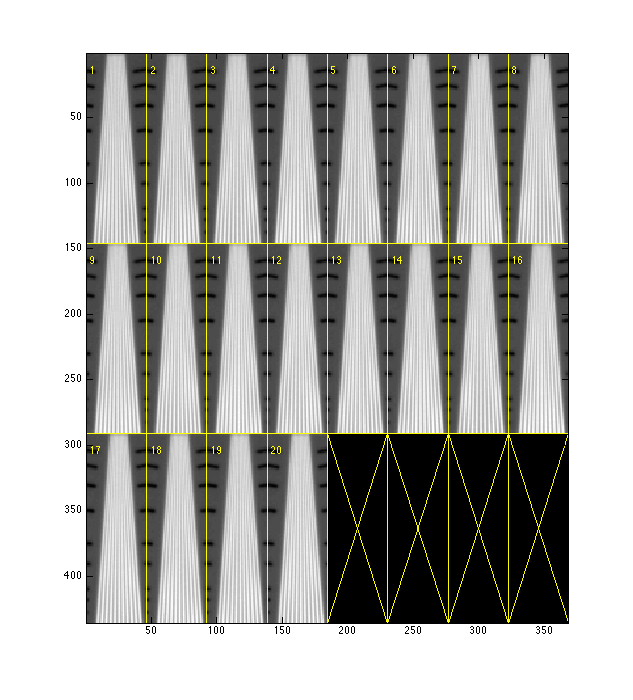
\includegraphics[width = 1.0\textwidth]{data_cropped}
\caption{Cropped low-resolution image sequence} \label{crop}
\end{figure}

To make sure the correctness of the computation and procedure, one can start with a simple toy problem. For example, one can start with
trying reconstruct a small single row. In this case, one can actually implement everything over a matrix base, since it's just a single row. It's easy to get things work using matrix form. Once we have that work, we have the ground truth, then we can refer the result of any step in matrix form, which help us locate errors in the functional form. 

\begin{figure}[H]
\centering
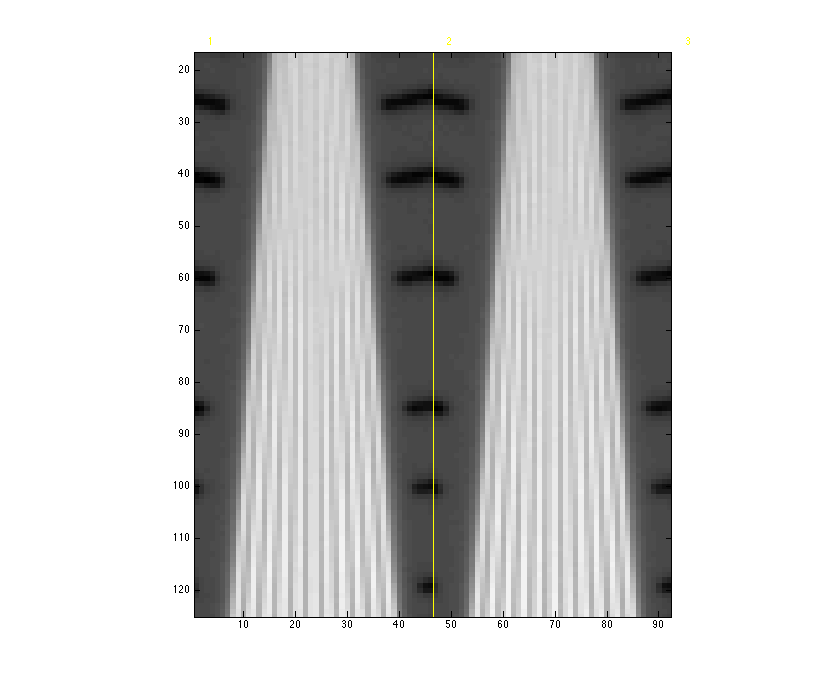
\includegraphics[width = 1\textwidth]{data_magnified}
\caption{Zoomed Cropped low-resolution image } \label{zoom}
\end{figure}

\begin{table}[h!]
\centering
\begin{tabular}{ | m{2cm}| m{2cm} | m{2cm} | m{2cm} |} 
\hline
 observe movement (pixel size)&  Real movement (pixel size)& Observe movement & Real movement \\ 
\hline
 0.1 & 0.14 & 1.0 & 1.14 \\ 
\hline
0.2 & 0.18 & 1.1 &  1.41\\ 
\hline
0.3 & 0.31& 1.2  & 1.48  \\ 
\hline
0.4 & 0.37&  1.3 &  1.75\\ 
\hline
0.5 & 0.53&  1.4 &  1.80\\ 
\hline
0.6 & 0.57& 1.5 & 2.04  \\ 
\hline
0.7 & 0.77& 1.6 & 2.08 \\ 
\hline
0.8 & 0.82&  1.7 & 2.29 \\ 
\hline
0.9 & 1.06&  1.8 &  2.34 \\ 
\hline
1.9 & 2.52&  - &  - \\ 
\hline
\end{tabular}
\caption{Acquiring movement and Real movement}
\label{table1}
\end{table}

The result of the iterated MAP estimation is shown in figure \ref{result} . Here, we reconstruct the image with a upsample factor = 2, i.e. each low resolution is the result of weighted average of two or three(if moved) high resolution pixel. In figure \ref{result}, the contrast and structure is much more clear on the upper part of line-pairs.

\begin{figure}[H]
\centering
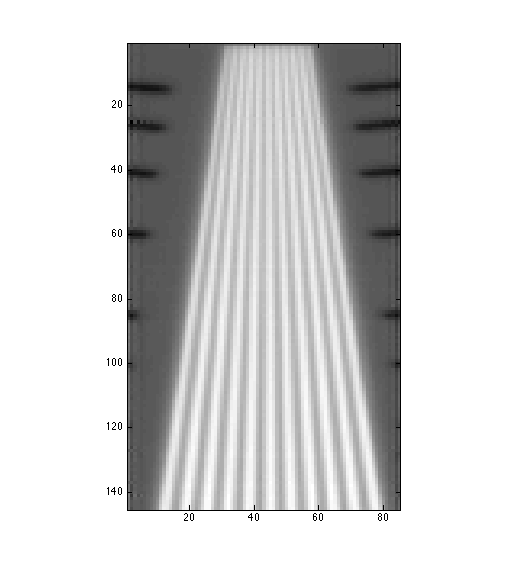
\includegraphics[width = 1\textwidth]{result}
\caption{MAP estimation of high resolution image (factor = 2)} \label{result}
\end{figure}

\section{Discussion}
The experiment only reconstruct the high resolution pixel along horizontal direction. It's might not be very difficult for 2D situations if we have already worked out 1D. In order to reconstruct images with 2D movement, we first need a sequence of low resolution images with both horizontal and vertical movements. Then we can use registration method to figure the the translation along both directions. Next, it seems we can do reconstructions by each direction independently. 

\section{Reference}
[1] Hardie, R. C., K. J. Barnard, and E. E. Armstrong. “Joint MAP Registration and High-Resolution Image Estimation Using a Sequence of Undersampled Images.” IEEE Transactions on Image Processing 6.12 (1997): 1621–1633. Web. 13 May 2016.

\newpage
\section{Code Appendix}
\lstinputlisting{/Users/whitefusion/Desktop/IndeStu/code/realdata_recon_main.m}
\lstinputlisting{/Users/whitefusion/Desktop/IndeStu/code/reconRow.m}
\lstinputlisting{/Users/whitefusion/Desktop/IndeStu/code/estimate_shift.m}
\lstinputlisting{/Users/whitefusion/Desktop/IndeStu/code/matrix_mult.m}
\lstinputlisting{/Users/whitefusion/Desktop/IndeStu/code/matrix_T_mult.m}

\end{document}